\section{Problems}
\label{section:conceptGenProblems}
\graphicspath{ {./chapter04/FigSolutions} }

\begin{enumerate}
\def\labelenumi{\arabic{enumi}.}
\item
  Consider the nine dot puzzle shown in Figure~\ref{figure:dotsProblems} (b). Draw
    \textbf{three} connected straight lines that pass through all nine
    dots.
    
    \begin{onlysolution}
    \textbf{[A]}
    \itshape
    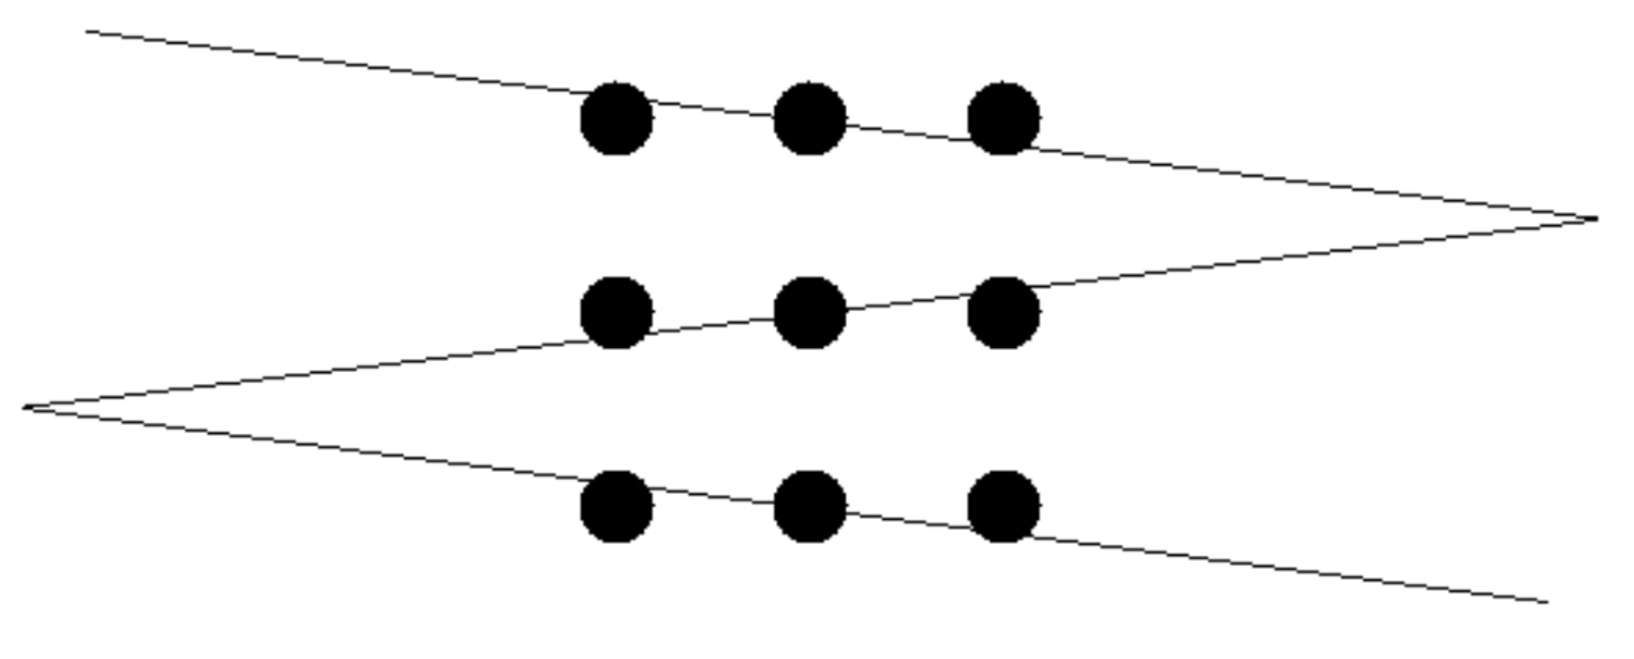
\includegraphics[width=0.8\textwidth]{image1}
  \end{onlysolution}

\item
  Consider the six sticks shown below. Rearrange the sticks to produce
  four equilat­eral triangles (the sticks cannot be broken).
  
  \begin{figure}[h]
    
\includegraphics[width=2in,height=1.35in]{../Fig/image35}
    \label{figure:sixSticks}
    \end{figure}

    \begin{onlysolution}
    \textbf{[A]}
    \itshape
    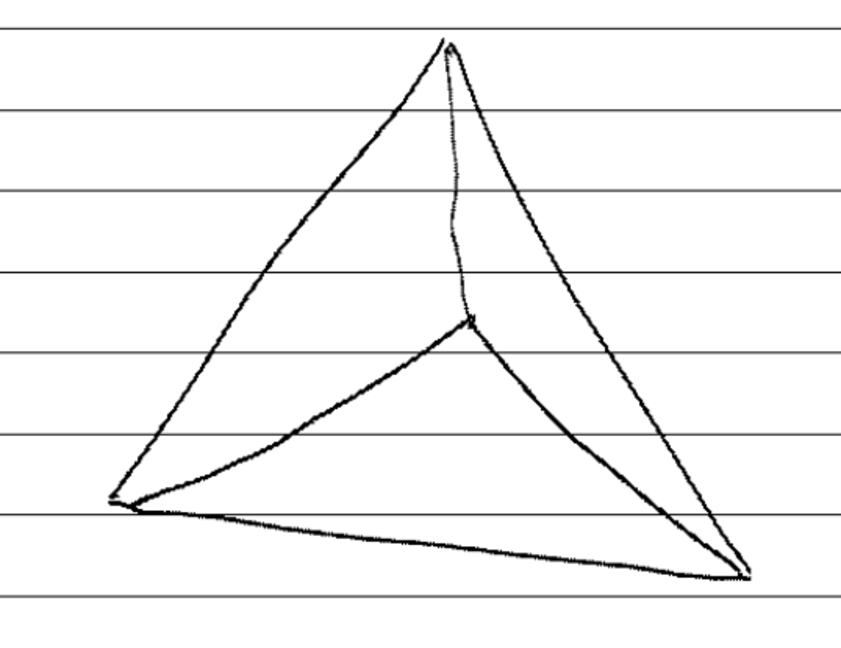
\includegraphics[width=0.8\textwidth]{image2} \\
    In this solutions, one has to go to 3 dimensions!
  \end{onlysolution}

\item
  Consider the fish shown below made of eight sticks and a coin for the
  eye. The objective is to make the fish face the other direction by
  moving only the coin and three sticks.

  \begin{figure}[h]
  
\includegraphics[width=2in,height=1.35in]{../Fig/image34}
  \label{figure:fishStickFigure}
  \end{figure}

  \begin{onlysolution}
    \textbf{[A]}
    \itshape
    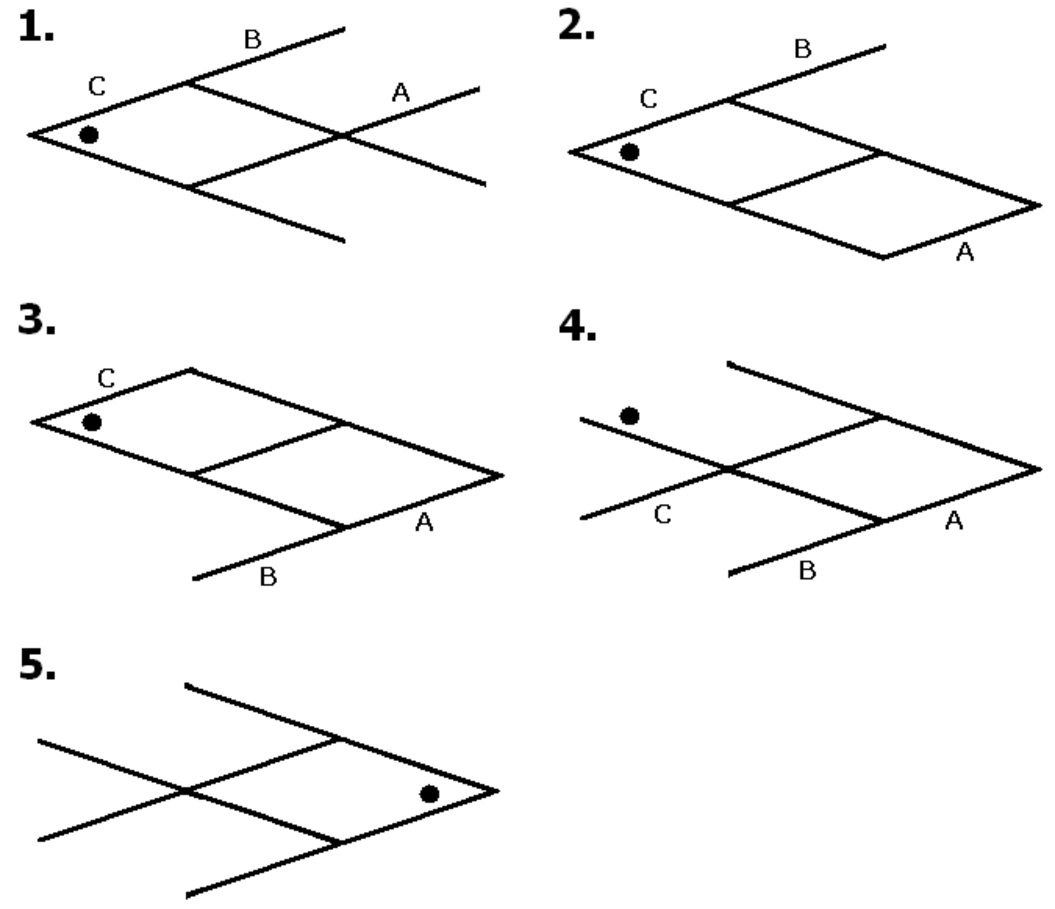
\includegraphics[width=0.8\textwidth]{image3}
  \end{onlysolution}

\item
  For each of the following lateral thinking puzzles, develop a
  plausible solution (from Paul Sloane's \ul{Lateral Thinking Puzzles}
  {[}http://dspace.dial.pipex.com/sloane{]}):

\begin{itemize}
\item
  A man walks into a bar and asks the barman for a glass of water. The
  barman pulls out a gun and points it at the man. The man says
  \textquotesingle Thank you\textquotesingle{} and walks out.

  \begin{onlysolution}
    \textbf{[A]}
    \itshape
    The man had hiccups. The barman recognized this from his speech and drew
    the gun in order to give him a shock. It worked and cured the hiccups - 
    so the man no longer needed the water.
  \end{onlysolution}

\item
  A woman had two sons who were born on the same hour of the same day of
  the same year. But they were not twins. How could this be so?

  \begin{onlysolution}
    \textbf{[A]}
    \itshape
    The woman had triplets. They were two of the triple.
  \end{onlysolution}

\item
  Why is it better to have round manhole covers than square ones?

  \begin{onlysolution}
    \textbf{[A]}
    \itshape
    While the square manhole sounds just as plausible as the round manhole cover, 
    there is a major disadvantage. The round manhole cover will never be able to 
    fall down the whole, because the diameter of the cover never changes. The square 
    cover, if in the right position, would be able to be dropped down the hole.
  \end{onlysolution}

\item
  A man went to a party and drank some of the punch. He then left early.
  Everyone else at the party who drank the punch subsequently died of
  poisoning. Why did the man not die?

  \begin{onlysolution}
    \textbf{[A]}
    \itshape
    The punch, in its original state, was not poisoned. So, the man that had 
    it early and left drank the punch without the poisoning. However, those 
    that stuck around at the party continued drinking the same punch even 
    after it was poisoned.
  \end{onlysolution}

\end{itemize}

\item
  Legislation was passed to allow handguns in the cockpits of passenger
  airliners to prevent hijacking. Brainstorm to develop concepts that
  prevent anyone other than the pilot from using the handgun.

  \begin{onlysolution}
    \textbf{[A]}
    \itshape
    \emph{Note:} This is a brainstorming exercise that we have used in 
    our class a number of times with good results. Many interesting solutions 
    will be developed, including those that involve biometric recognition of 
    people to match them with the gun, mechanical solutions, and electronic 
    solutions (i.e. proximity sensor of gun to pilot).
  \end{onlysolution}

\item
  Imagine if scientists and engineers were able to develop a technology
  that would allow people to be transported from any place on earth to
  another instantaneously. Brainstorm to determine the potential impact
  this would have on society.

  \begin{onlysolution}
    \textbf{[A]}
    \itshape
    Brainstorming - no solution provided
  \end{onlysolution}

\item
  Student advising at many colleges and universities is seen as an area
  that can be im­proved. Brainstorm to develop ideas as to how student
  advising could be improved at your college or university.

  \begin{onlysolution}
    \textbf{[A]}
    \itshape
    Brainstorming - no solution provided
  \end{onlysolution}

\item
  In your own words, describe what a concept table and a concept fan
  are.

  \begin{onlysolution}
    \textbf{[A]}
    \itshape
    A concept table is a methodic method of investigating different 
    combinations, arrangements, and substitutions of technologies for a 
    given design. A concept fan is a hierarchical graphical representation 
    of the design decisions, choices, and alternative solutions. A 
    disadvantage of them is that they assume a form, or architecture, 
    for the solution.
  \end{onlysolution}

\item
  Consider the problem solved in 
  Section~\ref{subsection:analytical-hierarchy-process-and-decision-matrices}. 
  For this example assume   that:
\begin{itemize}

\item
  The following is the result of the paired comparison.

\begin{table}
\begin{tabular}{|c|c|c|c|c|}
\hline
              &
Accuracy &
Cost &
Size &
Availability \\ \hline
Accuracy & 1 & 1/3 & 2 & ½ \\ \hline
Cost & 3 & 1 & 5 & 1 \\ \hline
Size & 1/2 & 1/5 & 1 & 2 \\ \hline
Availability & 2 & 1 & ½ & 1 \\ \hline
\end{tabular}
\end{table}


\item
  The parts costs are the following: resistors = \$0.05, bipolar
  transistors (BJTs) = \$0.10, op amps = \$0.35, and RTDs = \$0.25.
\item
  The parts have an in-stock availability of 99\%, 90\%, 85\%, and 70\%
  of the time for the re­sistors, BJTs, RTDs, and op amps respectively.
\item
  Everything else is the same as presented in 
  Section~\ref{subsection:analytical-hierarchy-process-and-decision-matrices}.
\end{itemize}

Compute the rankings of the design options using a weighted decision
matrix of the type shown in Table~\ref{table:pairwiseCompMatrix}.

  \begin{onlysolution}
    \textbf{[R]}
    \itshape
    
    \textul{Step 1: Determine the Criteria}
    In this example the comparison criteria of accuracy, cost, size and 
    availability were given as a part of the problem.
    
    \textul{Step 2: Select the Weighting Factors}
    The weighting factors for the criteria are selected based upon the 
    scores from the pair wise comparison. Normalizing the weighing factors 
    as indicated in (2) produces \textbf{$\omega_1$ = 1/6 = 0.17, $\omega_2$ = 2.5/6 = 0.42
    , $\omega_3$ = 0/6 = 0, $\omega_4$ = 2.5/6 = 0.42.} 
    
    \textul{Step 3: Select the Design Ratings}
    Design ratings need to be made for each of the criterion.
    \textit{Accuracy.} Since the objective is to minimize the deviation, 
    the following rating is used 
      ** figure ** 
    
    This produces the following design ratings for accuracy: $\alpha_{11}$ = 0.14, $\alpha_{12}$ = 1.0, 
    and $\alpha_{13}$ = 0.68; and normalizing the row sum produces \textbf{$\alpha_{11}$ = 0.08, $\alpha_{12}$ = 0.55, 
    and $\alpha_{13}$ = 0.37.}

    \textit{Cost.} Using the provided cost measure (\$0.40 for design 1, \$0.65 for design 
    2, and \$0.50 for design 3) gives the following cost ratings for the three options 
    respectively: $\alpha_{21}$ = 1.0, $\alpha_{22}$ = 0.62, and $\alpha_{23}$ = 0.8. Normalizing the row sum produces 
    \textbf{$\alpha_{21}$ = 0.41, $\alpha_{22}$ = 0.26, and $\alpha_{23}$ = 0.33.}

    \textit{Size.} The objective is to minimize size. Using a measure analogous to the given 
    space to manufacture each produces the following normalized decision ratings: 
    \textbf{$\alpha_{31}$ = 0.48, $\alpha_{32}$ = 0.31, and $\alpha_{33}$ = 0.21.}

    \textit{Availability.} A measure for the overall availability of parts to manufacture 
    each design is required. One way to measure this is to compute the probability that a 
    design will be able to be manufactured based upon the past history of part availability. 
    This is found by multiplying the availability of all individual components needed for 
    the design:

      P(design 1 can be produced) = (0.99)(0.85)(0.90) = 0.76\\
      P(design 2 can be produced) = (0.99)(0.85)(0.70) = 0.59\\
      P(design 3 can be produced) = (0.99)(0.85)(0.90)(0.90) = 0.68



    This produces the following normalized decision ratings for availability: 
    \textbf{$\alpha_{41}$ = 0.37, $\alpha_{42}$ = 0.29, and $\alpha_{43}$ = 0.33.}

    \textul{Step 4: Compute the Scores}
      ** add table **

    \textul{Step 5: Review the Decision}
    Remember that this is a semi-quantitative method. The final ranking indicates that design 
    all design options are essentially equal in this case.

      ** Add figures
  \end{onlysolution}

\item
  \textbf{Project Application.} Utilize the methods in this chapter to
  generate con­cepts for your particular design problem. Critically
  evaluate the concepts generated using one or more of the techniques
  presented in the chapter that is appropriate for the problem. 
  Section~\ref{section:project-application-concept-generation-and-evaluation}
  pro­vides guidance on how to conduct this process and document the
  results.

  \begin{onlysolution}
    \textbf{[R]}
    \itshape
    
    \textbf{Note:} We usually combine this with the Design project application problem (5.7) 
    in Chapter 5. What we are looking for is for each team to show that they have examined 
    different potential solutions to the design problem and evaluated the alternatives. 
    Thus they can document the results a variety of ways – such as concept fan/table or 
    decision matrix. Highly quantitative decision tables are frankly difficult to develop, 
    and the results may not be that valuable. We try to get them to demonstrate that they 
    have put serious effort into examining the different solutions for a problem. Below is 
    the text from the assignment that is provided to the students.

    The team must show that it has analyzed and evaluated different options/concepts for the 
    design. This means that you should have examined different alternatives and be able to 
    justify the choices the team made. The choices could be in terms of different design 
    architectures and/or different decisions for elements of the overall system.
    
    Apply the methods from Chapter 4 that are appropriate for the problem. The results can be 
    presented in terms of a list of brainstormed ideas, Concept Tables/Fans and Decision 
    matrices. If you do use decision matrices, you can use them to benchmark or compare different 
    technical solutions considered. Only use the highly quantitative matrix (i.e. Example 4.1) if 
    it realistic and applicable to the problem.
  \end{onlysolution}

\end{enumerate}

